\section{Langkah-Langkah Percobaan}
\subsection{Percobaan 1: Crimping Kabel UTP}
\begin{enumerate}
	\item Mengupas kabel UTP hingga terlihat kabel twisted pair.
	\item Meluruskan dan merapikan untaian kabel twisted pair. 
	\item Menyusun urutan kabel sesuai dengan urutan kabel pada konfigurasi straight through T568A.
	\item Memasukkan kabel ke dalam kepala RJ45, pastikan seluruh kabel dalam urutan yang benar dan sampai ke ujung RJ45.
	\item Memasukkan kepala RJ45 yang sudah dimasuki kabel ke dalam tang crimping lalu menekan tang hingga kabel tercrimping dengan benar.
	\item Menguji hasil crimping kabel dengan LAN tester.
\end{enumerate}
\subsection{Percobaan 2: Static Routing IPv4}
\begin{enumerate}
	\item Menyalakan router dan mereset router bila diperlukan.
	\item Melakukan login ke router
	\item Melakukan konfigurasi alamat IP pada router. Pada router pertama, interface ether1 diberi IP 192.168.10.1 dan interface ether2 diberi IP 10.10.10.2. Pada router kedua, interface ether1 diberi IP 192.168.20.1 dan interface ether2 diberi IP 10.10.10.1.
	\item Melakukan konfigurasi routing pada masing-masing router. Pada router pertama dilakukan konfigurasi routing statis dengan IP address 192.168.20.0 dan gateway 10.10.10.1. Pada router kedua dilakukan konfigurasi routing statis dengan IP address 192.168.10.0 dan gateway 10.10.10.2.
	\item Menghubungkan port eth2 router pertama dengan port eth2 router kedua menggunakan kabel UTP untuk membuat koneksi antar router.
	\item Menghubungkan port eth1 router dengan port LAN pada laptop.
	\item Melakukan konfigurasi IP statis pada laptop. Untuk laptop yang terhubung dengan router pertama, konfigurasi IP statis diatur menjadi 192.168.10.2. Untuk laptop yang terhubung dengan router kedua, konfigurasi IP statis diatur menjadi 192.168.20.2.
	\item Melakukan ping dari laptop pertama ke laptop kedua dan sebaliknya. Pada laptop pertama (yang tersambung dengan router pertama) dilakukan ping ke alamat 192.168.20.2, pada laptop kedua (yang terhubung dengan router kedua) dilakukan ping ke alamat 192.168.10.2.
\end{enumerate}
\subsection{Percobaan 3: Dynamic Routing IPv4}
\begin{enumerate}
	\item Menyalakan router dan mereset router bila diperlukan.
	\item Melakukan login ke router
	\item Mengaktifkan routing RIP pada router bila diperlukan.
	\item Melakukan konfigurasi alamat IP pada router. Pada router pertama, interface ether1 diberi IP 192.168.10.1 dan interface ether2 diberi IP 10.10.10.2. Pada router kedua, interface ether1 diberi IP 192.168.20.1 dan interface ether2 diberi IP 10.10.10.1.
	\item Melakukan konfigurasi server DHCP pada masing-masing router dan menyesuaikan interfacenya dengan interface yang digunakan untuk menghubungkan router dengan laptop (pada percobaan ini adalah ether1).
	\item Melakukan konfigurasi routing dinamis pada masing-masing router menggunakan RIP. Pada semua router konfigurasi bagian interfaces menjadi ether all. Pada router pertama bagian networks ditambahkan alamat 10.10.10.0 dan 192.168.10.0 dan pada router kedua bagian networks ditambahkan alamat 10.10.10.0 dan 192.168.20.0. Pada router pertama bagian neighours ditambahkan alamat 192.168.20.0 dan pada router kedua bagian neighbours ditambahkan alamat 192.168.10.0.
	\item Menghubungkan port eth2 router pertama dengan port eth2 router kedua menggunakan kabel UTP untuk membuat koneksi antar router.
	\item Menghubungkan port eth1 router dengan port LAN pada laptop.
	\item Melakukan konfigurasi IP dinamis pada laptop. Konfigurasi dilakukan cukup dengan mengubah pengaturan IP dari statis ke DHCP.
	\item Melakukan ping dari laptop pertama ke laptop kedua dan sebaliknya. Untuk mengetahui alamat IP yang diberikan oleh server DHCP, dapat dilakukan dengan menggunakan perintah ipconfig pada cmd atau powershell.
\end{enumerate}

\section{Analisis Hasil Percobaan}
Pada percobaan pertama, dilakukan crimping kabel UTP dengan konfigurasi straight-through dan urutan warna T568A. Setelah dilakukan crimping, kabel akan dites menggunakan LAN tester. Secara teori, bila konfigurasi crimping kabel benar, maka lampu pada LAN tester semuanya akan menyala secara berurutan dan sinkron antara sisi kanan dan sisi kiri. Pada pengujian pertama, ada lampu LAN tester yang tidak menyala pada satu sisi. Setelah diperiksa, ternyata pada salah satu sisi kabel, tidak semua kabel mennyentuh ujung kepala RJ45 sehingga kabel tidak terhubung dengan RJ45 dan lampu tidak menyala. Karena kesalahan ini, maka dilakukan crimping ulang. Pada pengujian kedua, semua lampu LAN tester menyala dan semuanya berurutan dan sinkron antaea kedua sisi. Hasil pengujian LAN tester ini membuktikan bahwa konfigurasi dan urutan kabel saat crimping telah benar.
\\
\indent
Pada percobaan kedua, dilakukan routing statis IPv4. Secara teori, saat komputer melakukan ping kepada sebuah alamat IP, maka ping tersebut akan mencari host dengan alamat IP tersebut di dalam jaringan, dan bila alamat IP ada di router lain maka pencarian akan diteruskan ke router yang memiliki alamat IP tersebut melalui gateway router. Bila routing statis berhasil, maka kedua laptop akan dapat melakukan ping ke alamat IP satu sama lain yang telah ditetapkan pada pengaturan IP. Hasil akhir yang didapatkan setelah melakukan konfigurasi routing statis dan melakukan ping adalah kedua laptop dapat melakukan ping ke alamat IP satu sama lain. Laptop pertama dengan IP statis 192.168.10.2 dapat melakukan ping ke laptop kedua dengan IP statis 192.168.20.2, begitu pula sebaliknya. Hasil ini membuktikan bahwa percobaan telah dilakukan dengan benar dan cocok antara teori dengan hasil akhir percobaan.
\begin{figure}[H]
	\centering
	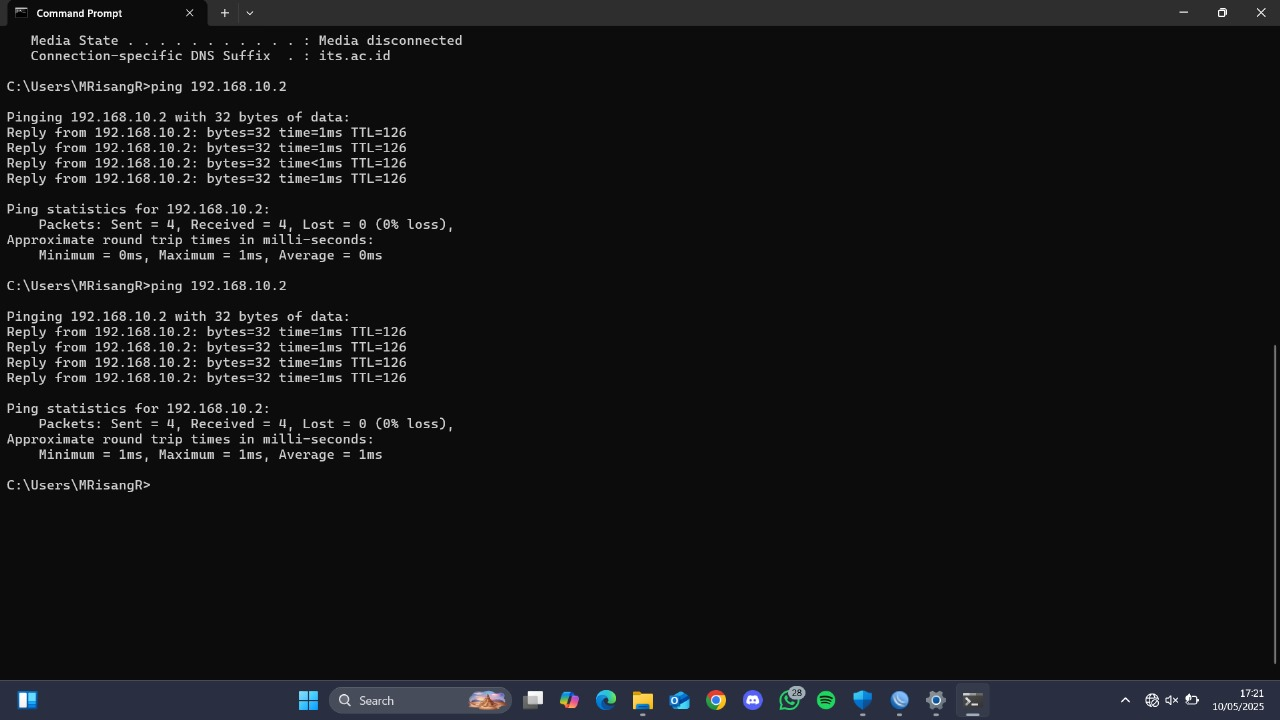
\includegraphics[scale=0.5]{P1/img/ping 10.2.jpg}
	\caption{Ping dari laptop 1 ke laptop 2}
\end{figure}
\begin{figure}[H]
	\centering
	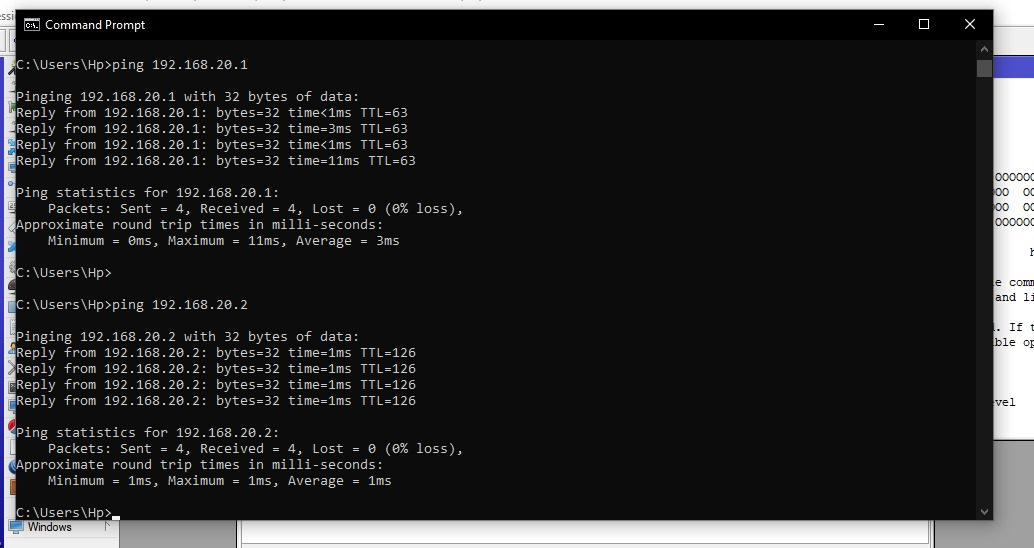
\includegraphics[scale=0.55]{P1/img/ping 20.2.jpg}
	\caption{Ping dari laptop 2 ke laptop 1}
\end{figure}

Pada percobaan ketida, dilakukan routing dinamis IPv4. Secara teori, dengan routing dinamis menggunakan DHCP, maka pengaturan alamat IP hanya perlu dilakukan pada router yang bertindak sebagai server DHCP dan host lain seperti komputer hanya perlu dihubungkan ke jaringan tanpa harus melakukan konfigurasi IP secara manual karena alamat IP telah diberikan secara otomatis oleh server DHCP. Bila routing dinamis berhasil, maka kedua laptop yang digunakan dalam percobaan akan mampu melakukan ping satu sama lain menggunakan alamat IP yang diberikan seara otomatis oleh server DHCP. Hasil akhir pada percobaan ini adalah tidak ada laptop yang mampu melakukan ping ke laptop lainnya. Percobaan disimpulkan gagal karena pada cmd, setelah melakukan perintah ping muncul reply dari router yang berbunyi destination net unreachable. Dengan adanya reply message ini dari router, maka masalah penyebab kegagalan kemungkinan besar karena kesalahan pada pengaturan gateway router, karena bila router menyampaikan reply destination net unreachable itu artinya alamat IP yang dituju tidak bisa dicapai/dicari oleh router, sedangkan secara teori bila konfigurasi IP address dan gateway router sudah benar maka seharusnya router mampu mencapai alamat IP tujuan ping. Karena reply dari router sudah menunjukkan alamat IP router yang benar, yaitu alamat IP router yang terhubung dengan laptop, maka dapat disimpulkan bahwa konfigurasi yang salah ada pada konfigurasi gateway router.
\begin{figure}[H]
	\centering
	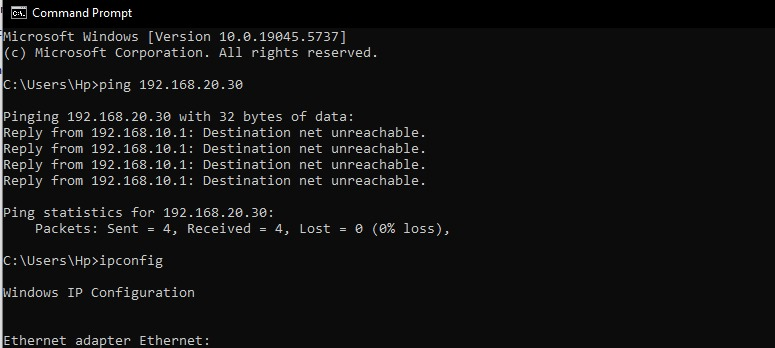
\includegraphics[scale=0.55]{P1/img/ping dhcp 10.1.jpg}
	\caption{Ping gagal dari laptop 1 ke laptop 2}
\end{figure}
\begin{figure}[H]
	\centering
	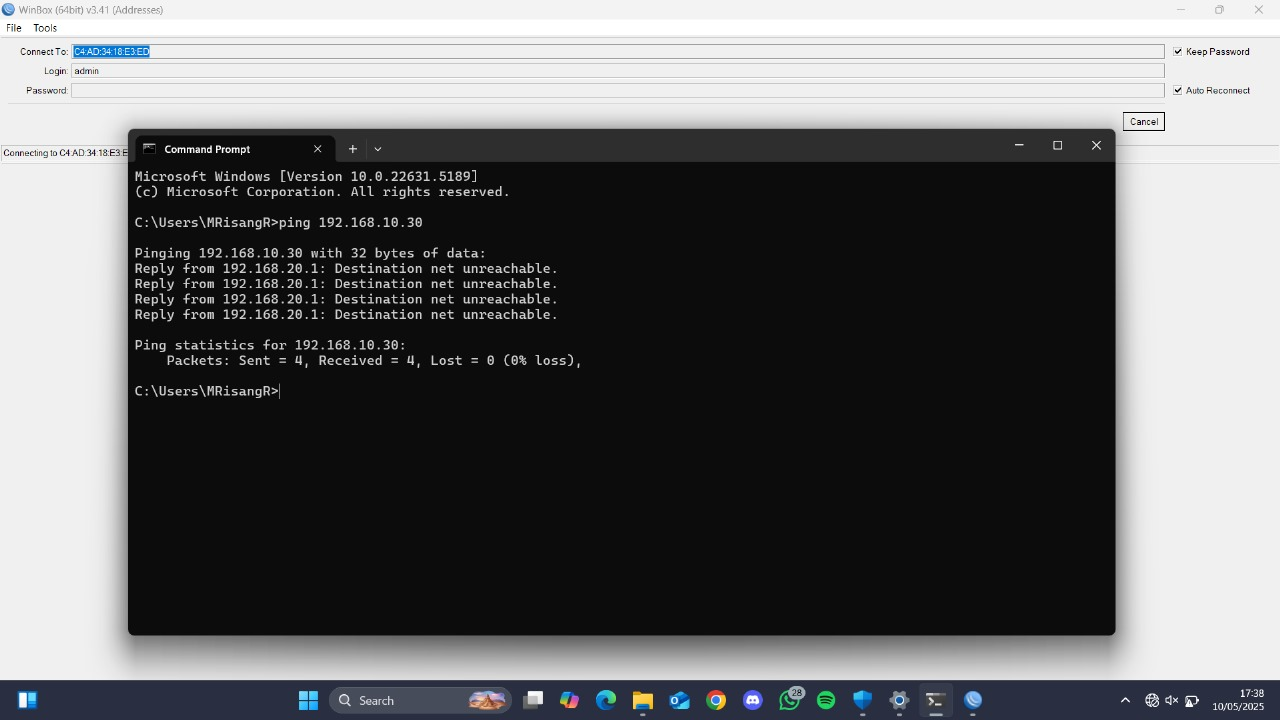
\includegraphics[scale=0.5]{P1/img/ping dhcp 20.1.jpg}
	\caption{Ping gagal dari laptop 1 ke laptop 2}
\end{figure}

\section{Hasil Tugas Modul}
\begin{enumerate}
	\item Berikut merupakan topologi jaringan yang sudah dikonfigurasi dan disimulasikan menggunakan cisco packet tracer. Pada gambar yang dilampirkan, dicontohkan koneksi antara PC14 dengan alamat IP 192.168.0.2 di departemen R\&D melakukan ping ke PC10 dengan alamat IP 192.168.0.131 di departemen produksi. Pada topologi ini, digunakan rasio 1:10, sehingga 50 perangkat milik departemen produksi diwakili 5 PC, 100 perangkat milik R\&D diwakili 10 PC, dan seterusnya.
	\begin{figure}[H]
		\centering
		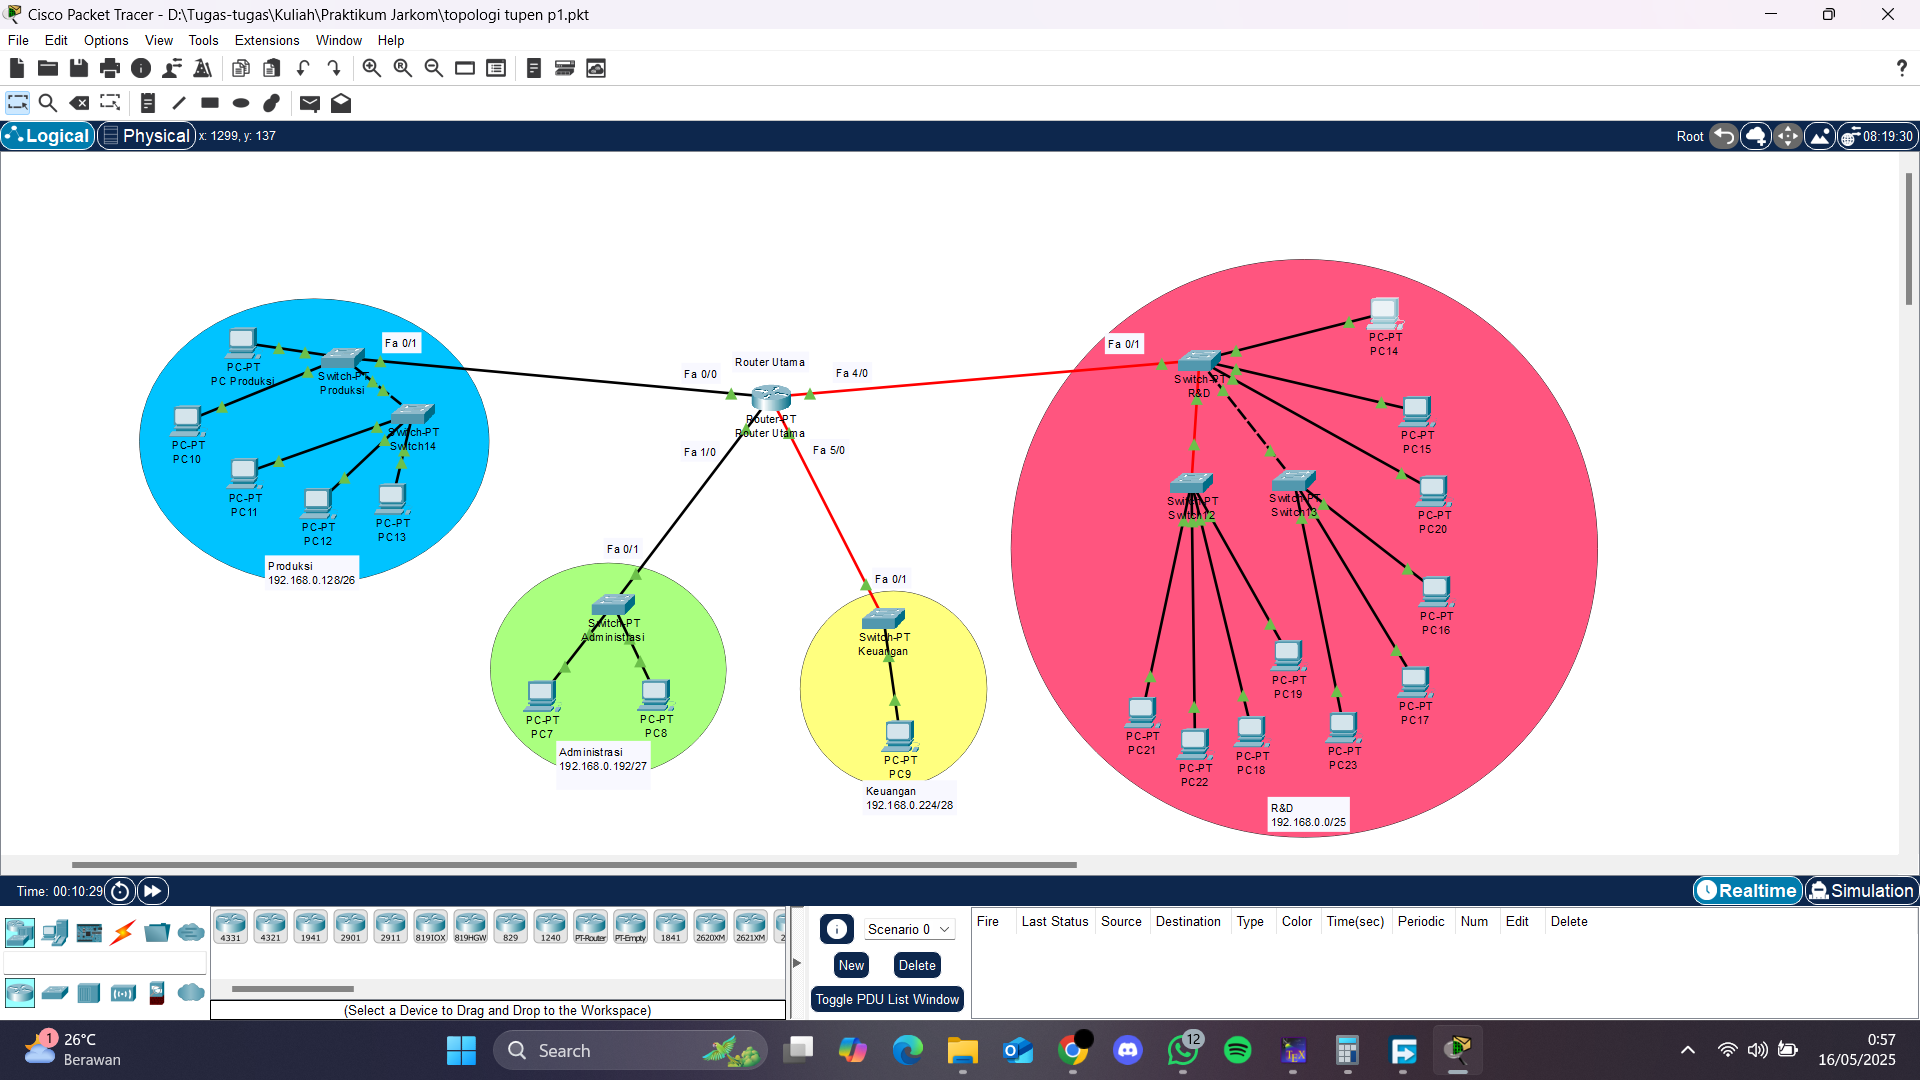
\includegraphics[scale=0.25]{P1/img/tupen topo.png}
		\caption{Topologi yang disimulasikan pada Cisco Packet Tracer}
	\end{figure}
	\begin{figure}[H]
		\centering
		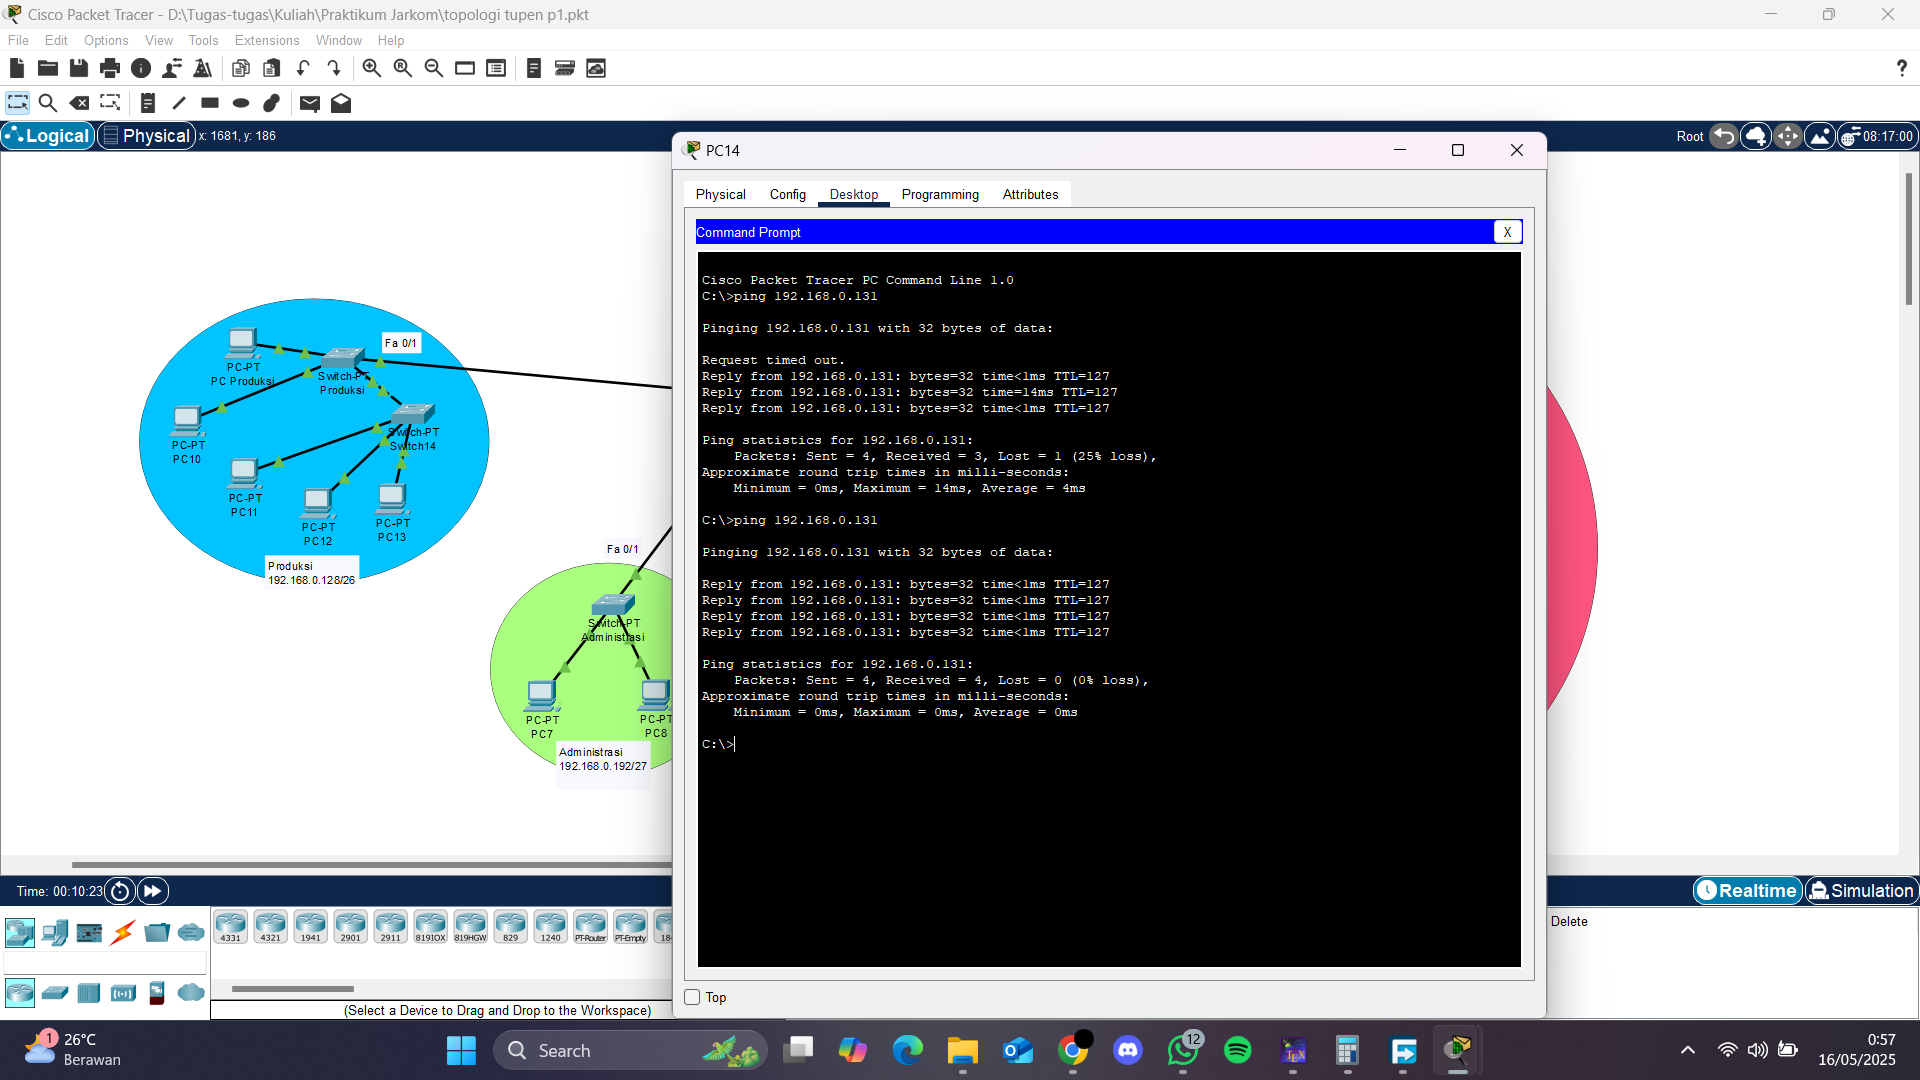
\includegraphics[scale=0.25]{P1/img/tupen ping.png}
		\caption{Ping dari PC14 dengan IP IP 192.168.0.2 ke PC10 dengan IP IP 192.168.0.131}
	\end{figure}
\end{enumerate}

\section{Kesimpulan}
Berdasarkan hasil pada percobaan pertama, dapat disimpulkan bahwa konfigurasi dan urutan kabel serta kepastian bahwa kabel sudah benar-benar terhubung ke kepala RJ45 adalah hal penting dalam crimping kabel UTP, karena bila konfigurasi kabel salah urutan maka LAN tester akan gagal karena urutan nyala lampu tidak sinkron, dan bila kabel tidak benar-benar terhubung ke kepala RJ45 maka LAN tester akan gagal karena lampu tidak menyala, sehingga diperlukan konfigurasi yang benar dan kabel yang benar-benar terhubung ke RJ45 agar kabel hasil crimping dapat digunakan dalam jaringan komputer. Berdasarkan hasil percobaan kedua, dapat disimpulkan bahwa routing statis berhasil dan sesuai dengan teori, karena kedua laptop yang digunakan dalam percobaan dapat melakukan ping ke satu sama lain. Berdasarkan hasil percobaan ketiga, dapat disimpulkan bahwa hasil percobaan tidak sesuai dengan teori. Namun, walaupun pada percobaan ini hasil tidak sesuai dengan teori, bukan berarti teori routing dinamis salah. Hal ini dikarenakan penyebab kegagalan ada pada kesalahan konfigurasi gateway pada router, sehingga laptop yang digunakan dalam percobaan gagal melakukan ping ke satu sama lain. Perbaikan pada konfigurasi juga tidak sempat dilakukan karena durasi praktikum sudah habis. Maka, pelajaran yang dapat diambil dari kegagalan percobaan ketiga adalah untuk lebih cepat dalam proses pengerjaan praktikum, agar bila terjadi masalah seperti kesalahan konfigurasi masih ada waktu untuk memperbaiki kesalahan tersebut dan mendapatkan hasil yang benar sesuai dengan teori.

\section{Lampiran}
\subsection{Dokumentasi saat praktikum}
\begin{figure}[H]
	\centering
	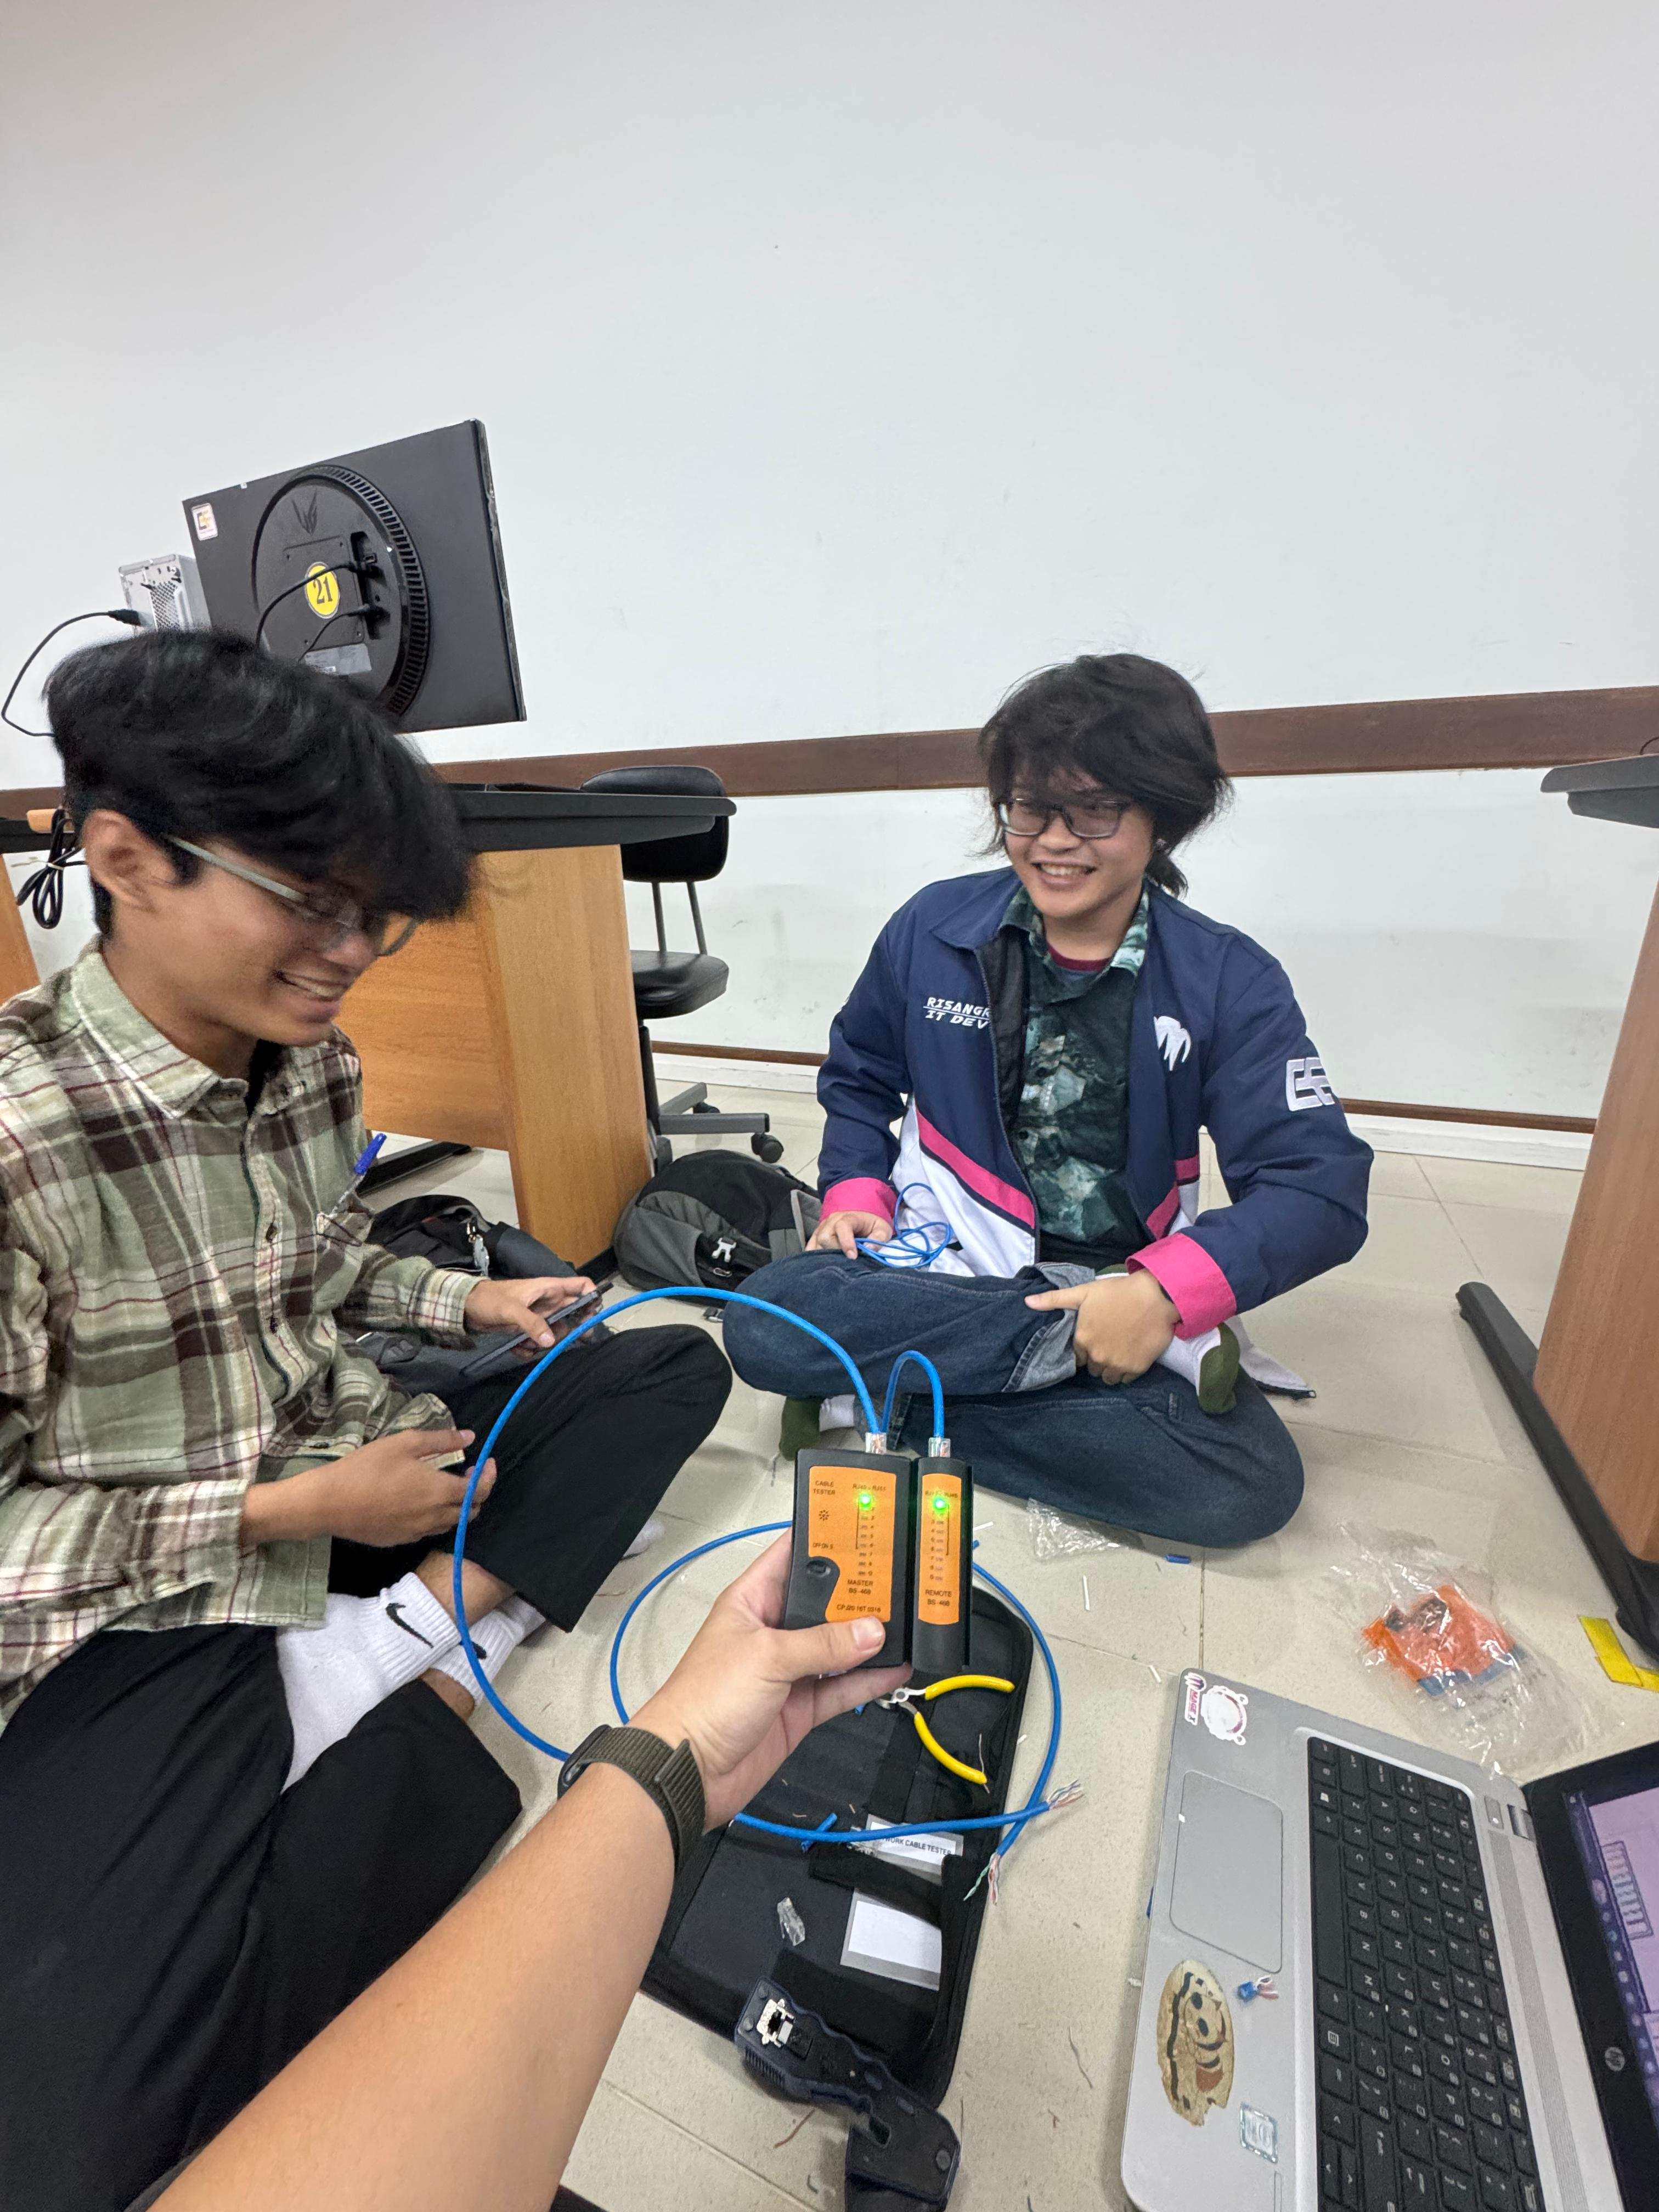
\includegraphics[scale=0.05]{P1/img/dokum1.jpg}
\end{figure}
\begin{figure}[H]
	\centering
	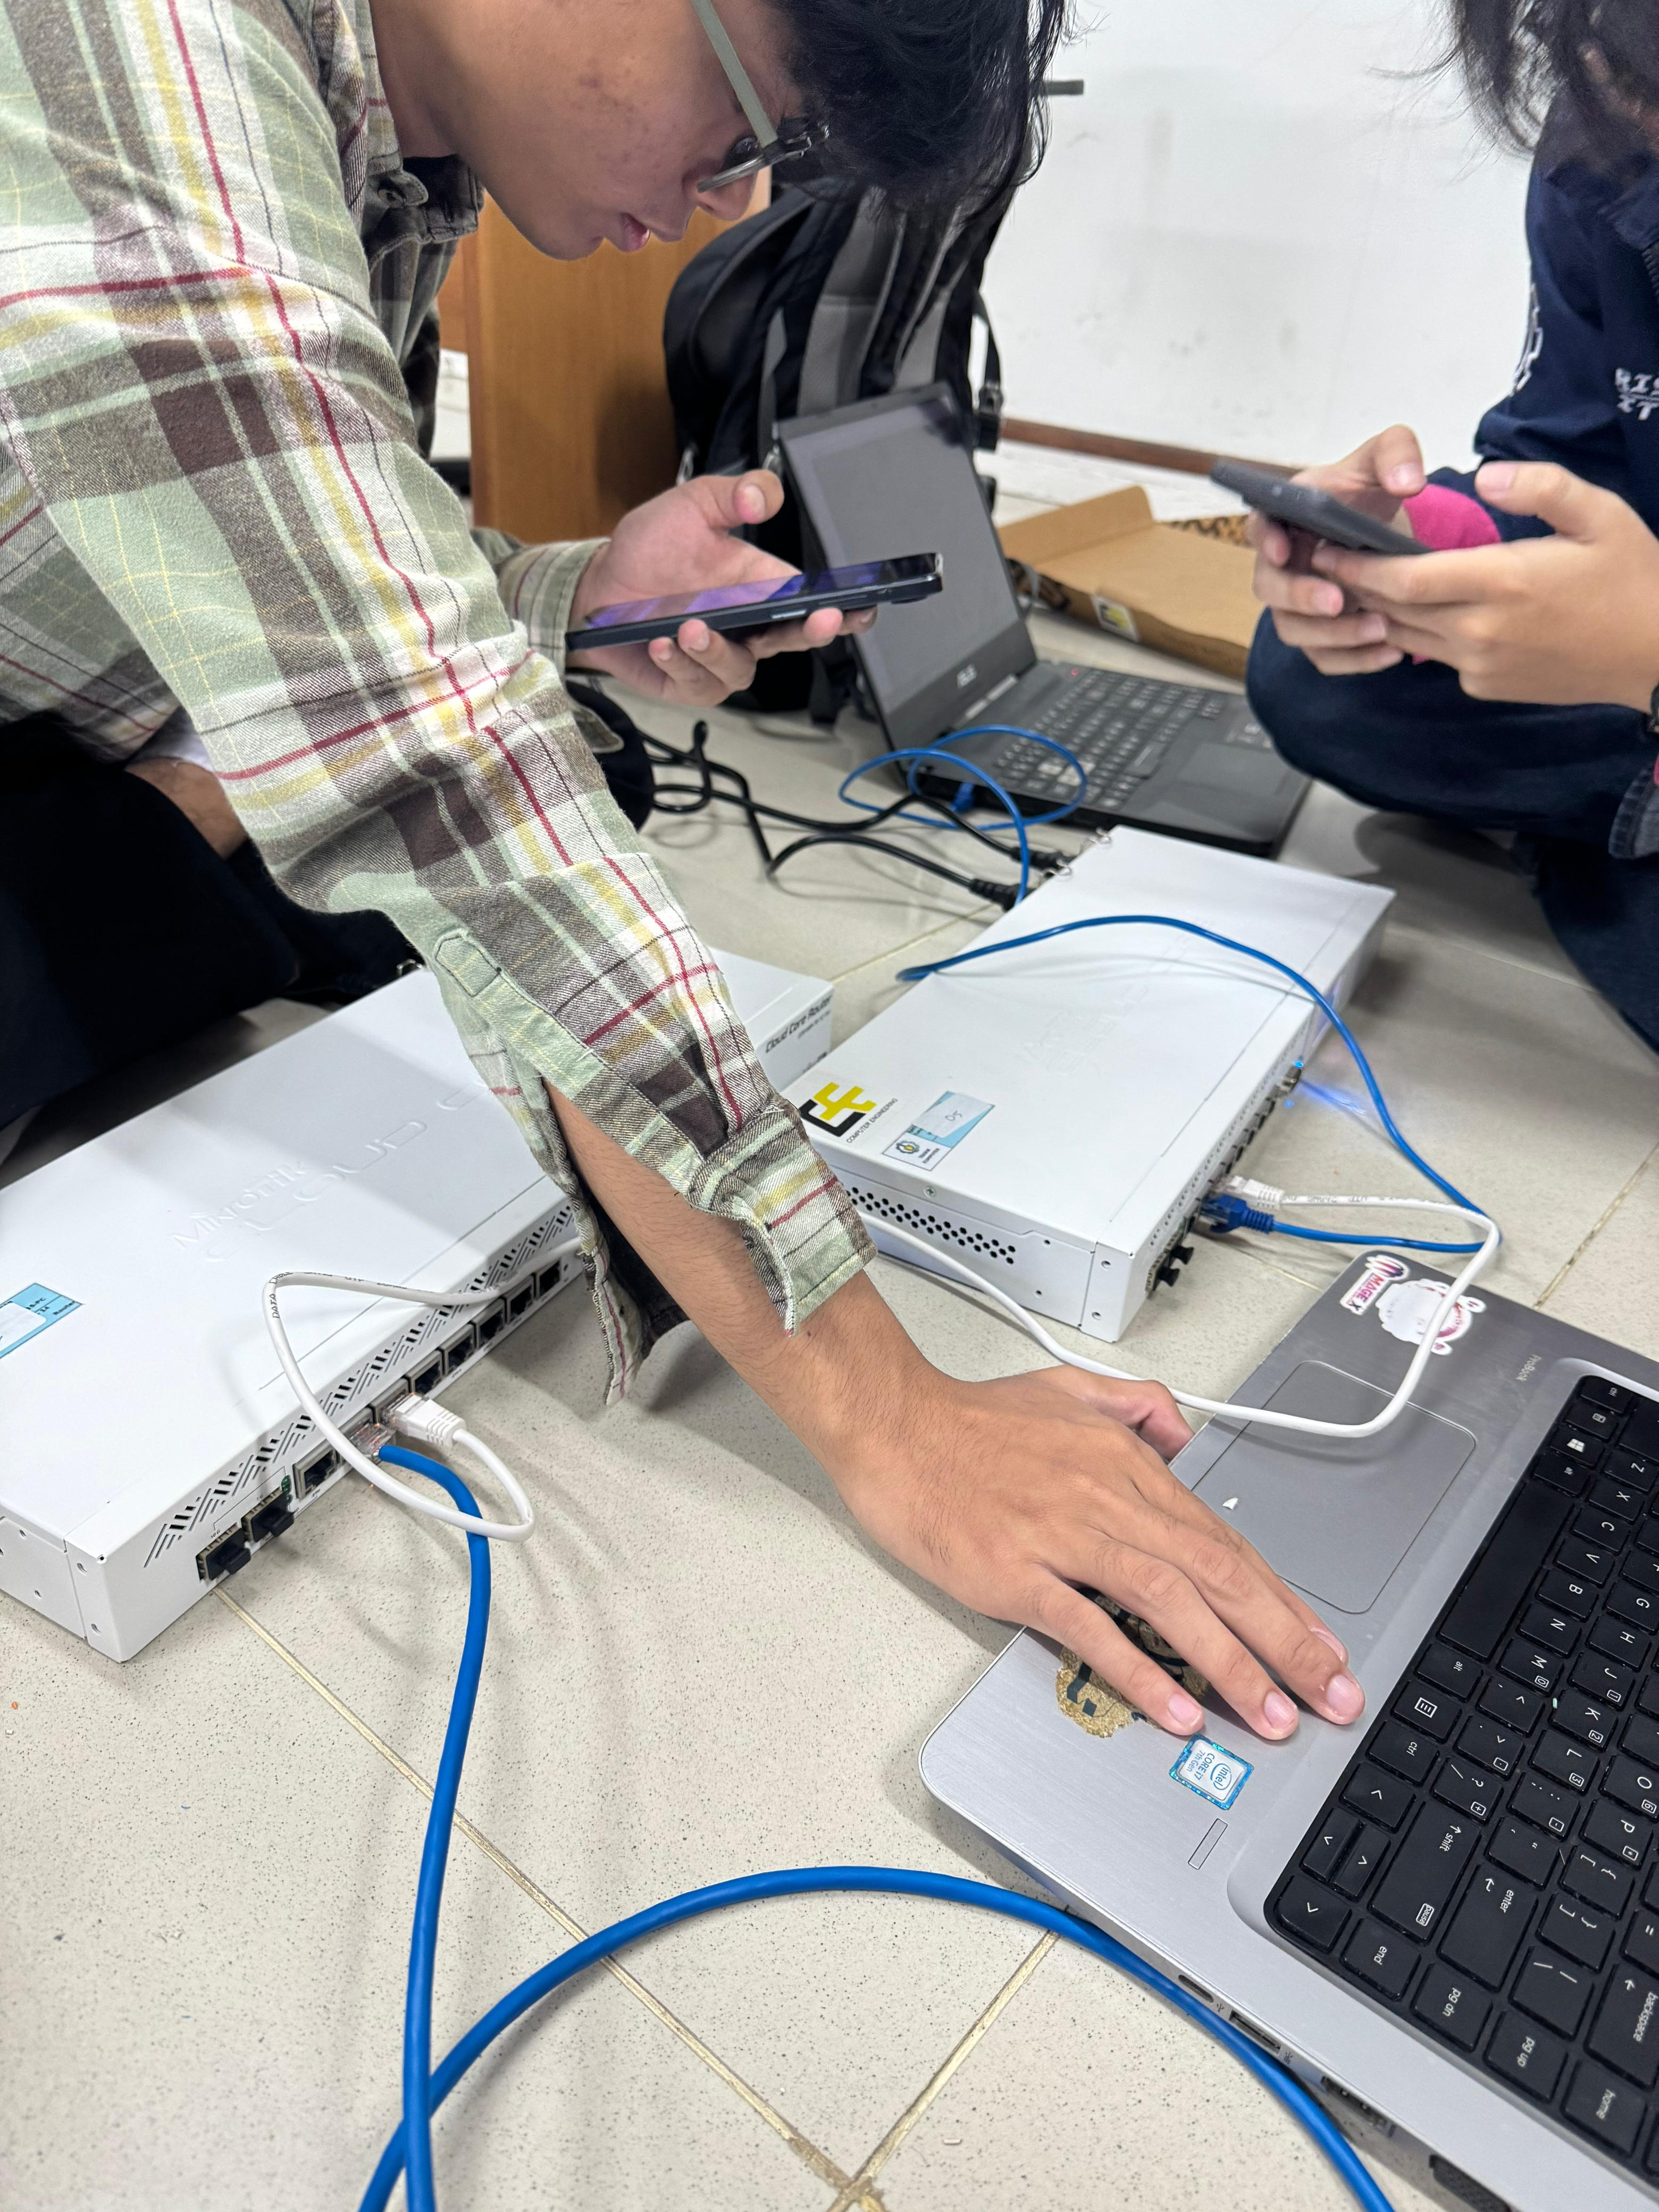
\includegraphics[scale=0.05]{P1/img/dokum2.jpg}
\end{figure}
\begin{figure}[H]
	\centering
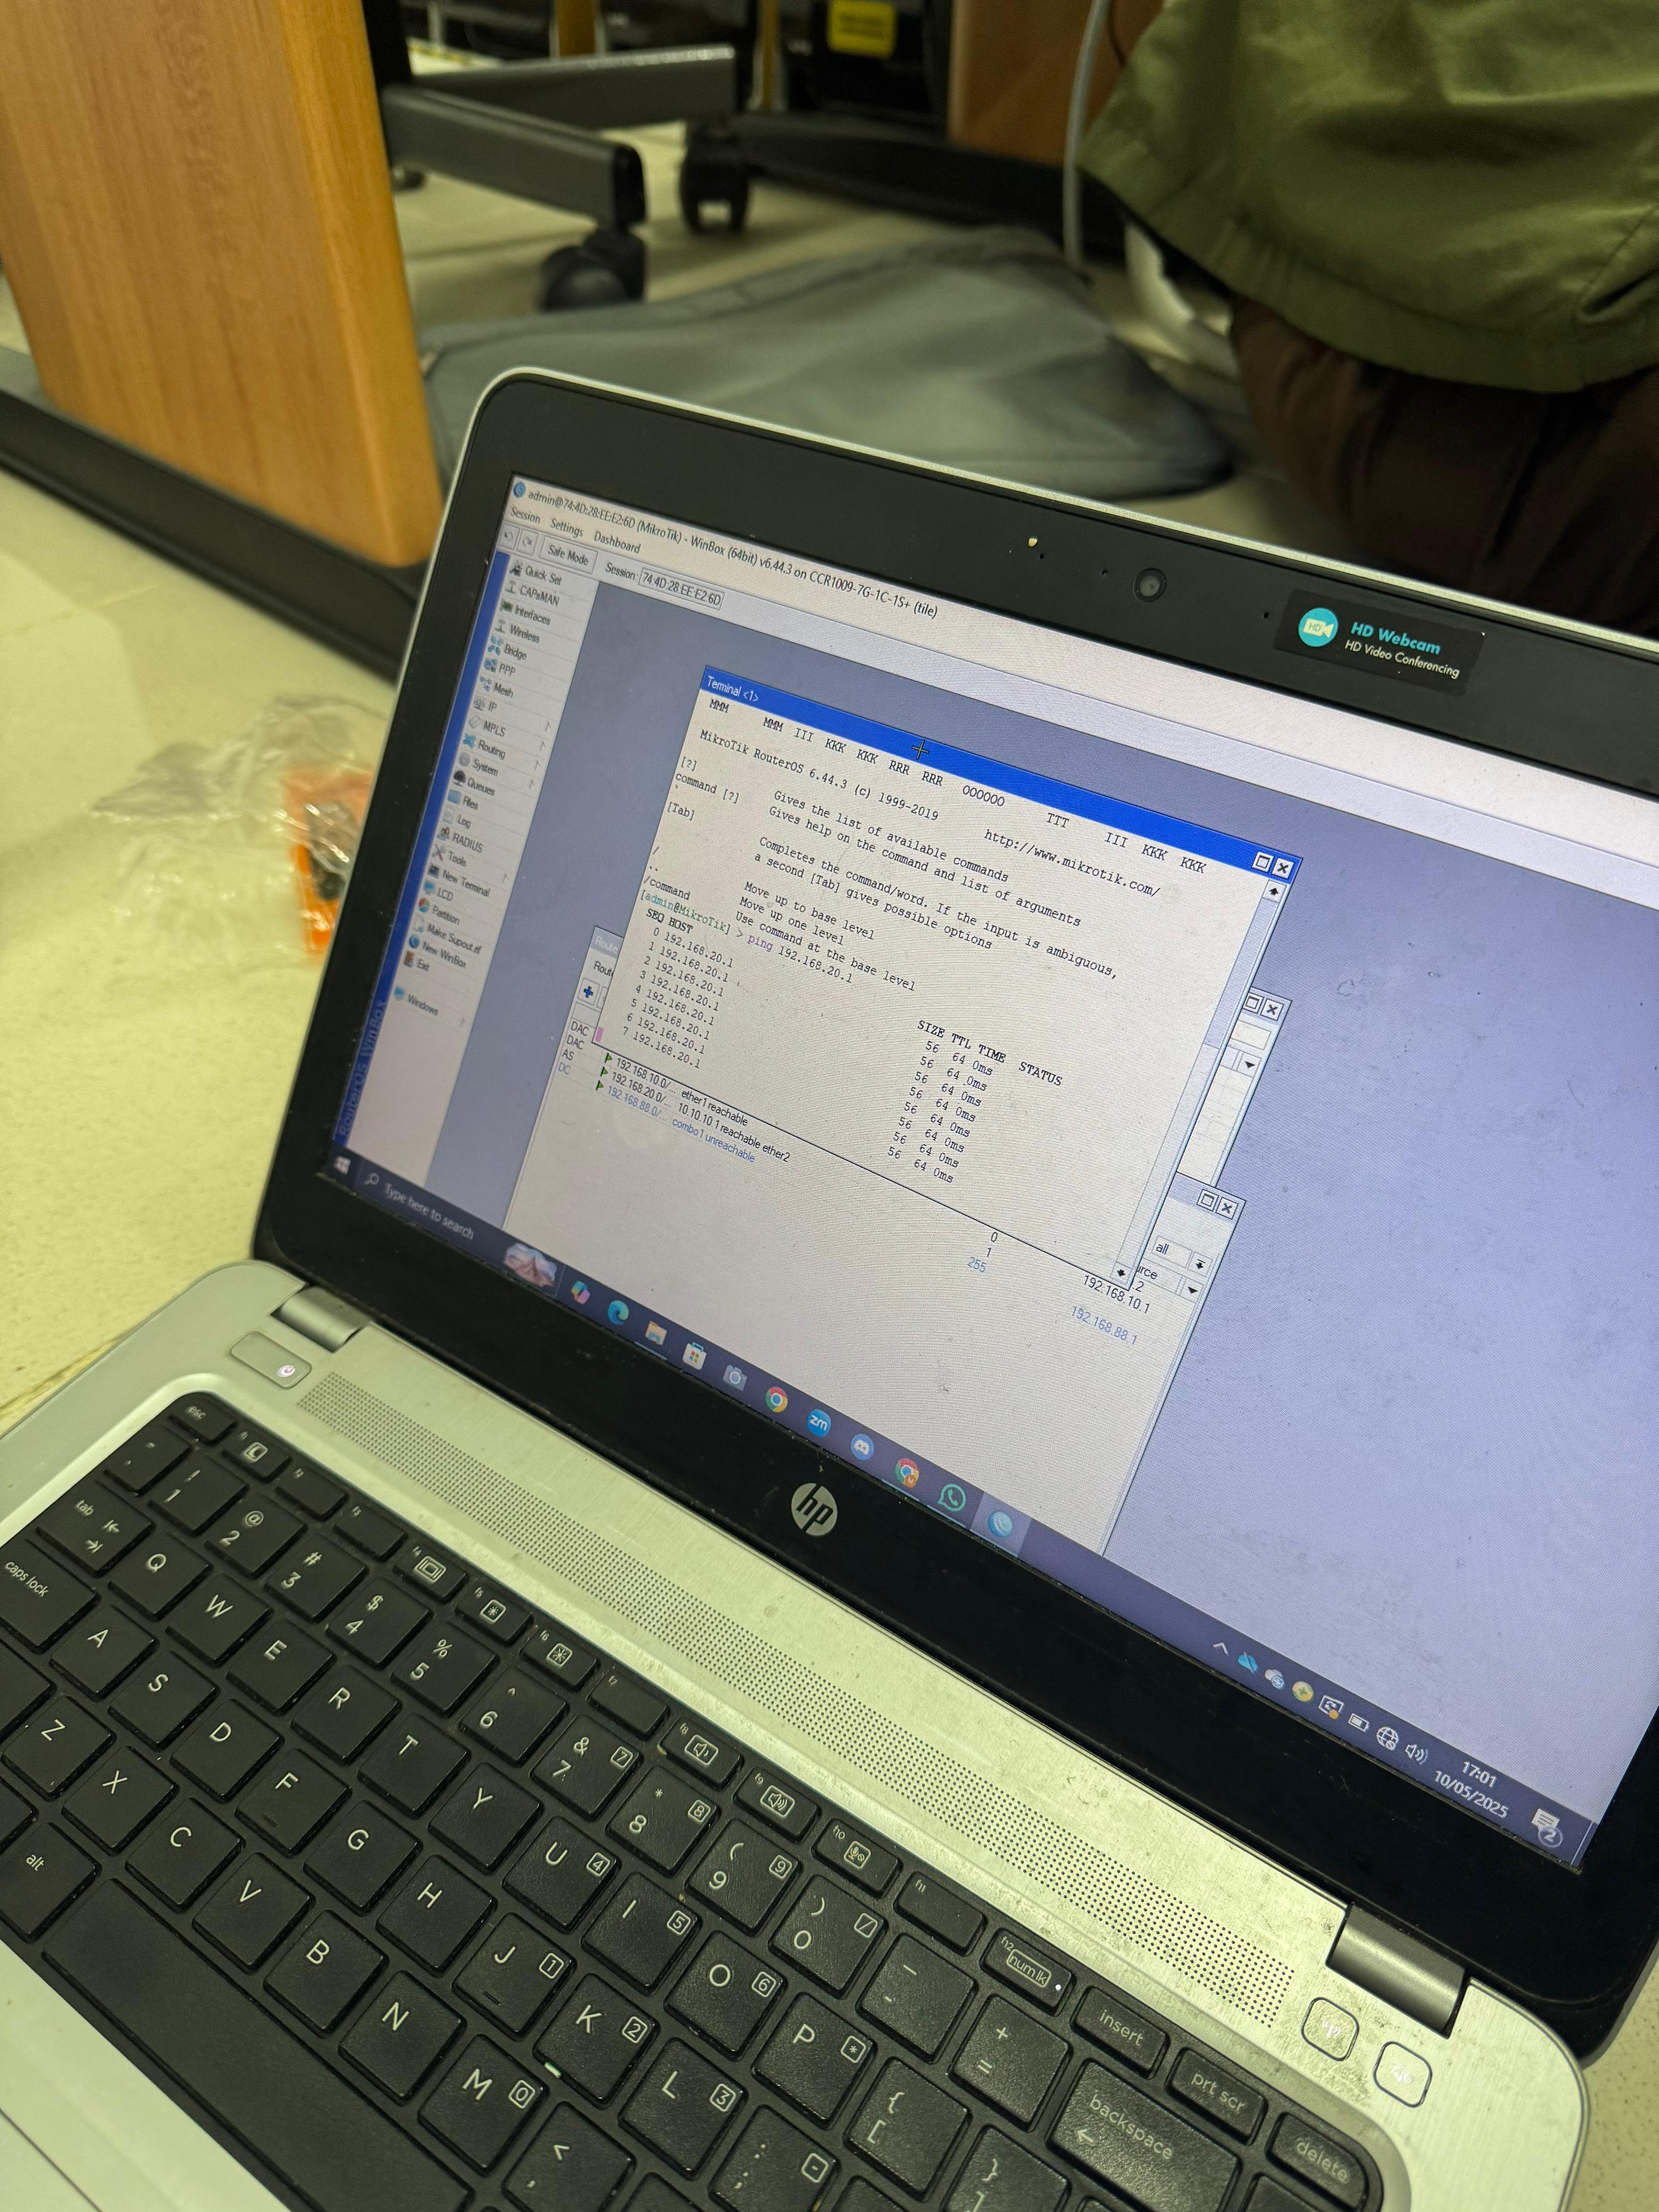
\includegraphics[scale=0.05]{P1/img/dokum3.jpg}
\end{figure}
\begin{figure}[H]
	\centering
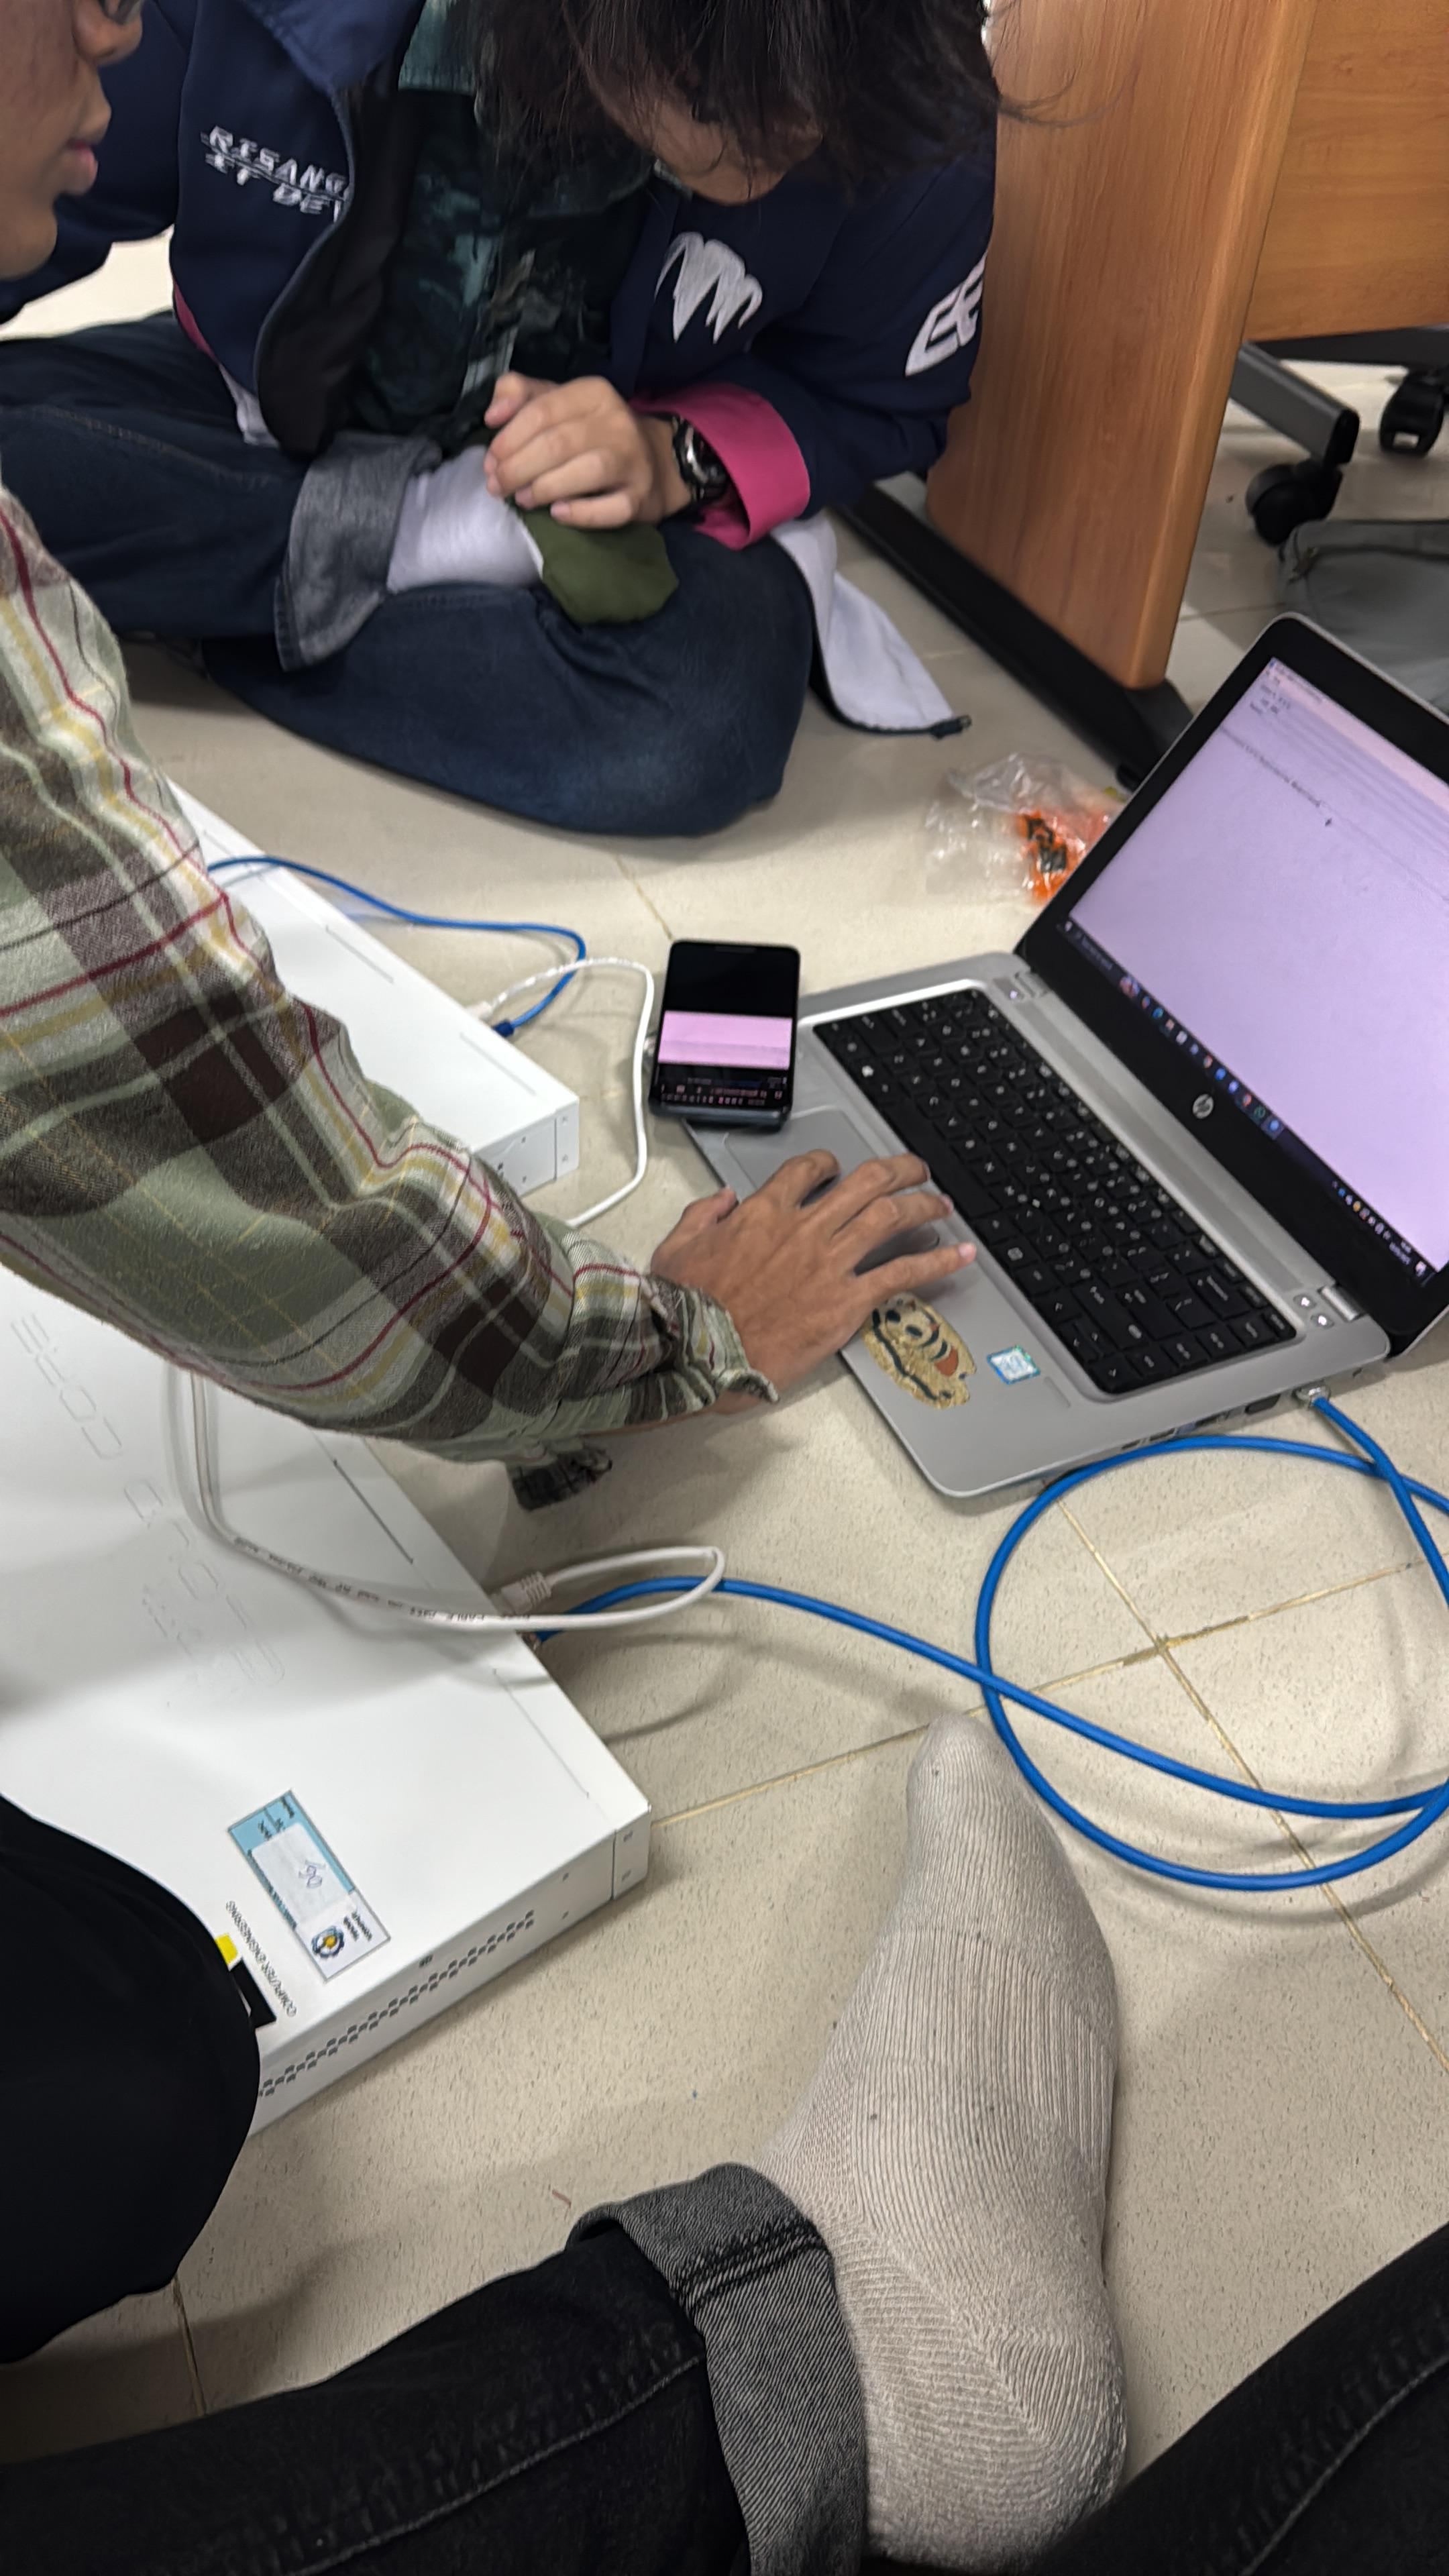
\includegraphics[scale=0.05]{P1/img/dokum4.jpg}
\end{figure}
